\PassOptionsToPackage{unicode=true}{hyperref} % options for packages loaded elsewhere
\PassOptionsToPackage{hyphens}{url}
%
\documentclass[ignorenonframetext,]{beamer}
\usepackage{pgfpages}
\setbeamertemplate{caption}[numbered]
\setbeamertemplate{caption label separator}{: }
\setbeamercolor{caption name}{fg=normal text.fg}
\beamertemplatenavigationsymbolsempty
% Prevent slide breaks in the middle of a paragraph:
\widowpenalties 1 10000
\raggedbottom
\setbeamertemplate{part page}{
\centering
\begin{beamercolorbox}[sep=16pt,center]{part title}
  \usebeamerfont{part title}\insertpart\par
\end{beamercolorbox}
}
\setbeamertemplate{section page}{
\centering
\begin{beamercolorbox}[sep=12pt,center]{part title}
  \usebeamerfont{section title}\insertsection\par
\end{beamercolorbox}
}
\setbeamertemplate{subsection page}{
\centering
\begin{beamercolorbox}[sep=8pt,center]{part title}
  \usebeamerfont{subsection title}\insertsubsection\par
\end{beamercolorbox}
}
\AtBeginPart{
  \frame{\partpage}
}
\AtBeginSection{
  \ifbibliography
  \else
    \frame{\sectionpage}
  \fi
}
\AtBeginSubsection{
  \frame{\subsectionpage}
}
\usepackage{lmodern}
\usepackage{amssymb,amsmath}
\usepackage{ifxetex,ifluatex}
\usepackage{fixltx2e} % provides \textsubscript
\ifnum 0\ifxetex 1\fi\ifluatex 1\fi=0 % if pdftex
  \usepackage[T1]{fontenc}
  \usepackage[utf8]{inputenc}
  \usepackage{textcomp} % provides euro and other symbols
\else % if luatex or xelatex
  \usepackage{unicode-math}
  \defaultfontfeatures{Ligatures=TeX,Scale=MatchLowercase}
\fi
% use upquote if available, for straight quotes in verbatim environments
\IfFileExists{upquote.sty}{\usepackage{upquote}}{}
% use microtype if available
\IfFileExists{microtype.sty}{%
\usepackage[]{microtype}
\UseMicrotypeSet[protrusion]{basicmath} % disable protrusion for tt fonts
}{}
\IfFileExists{parskip.sty}{%
\usepackage{parskip}
}{% else
\setlength{\parindent}{0pt}
\setlength{\parskip}{6pt plus 2pt minus 1pt}
}
\usepackage{hyperref}
\hypersetup{
            pdftitle={Livestock Breeding and Genomics},
            pdfauthor={Peter von Rohr},
            pdfborder={0 0 0},
            breaklinks=true}
\urlstyle{same}  % don't use monospace font for urls
\newif\ifbibliography
\usepackage{longtable,booktabs}
\usepackage{caption}
% These lines are needed to make table captions work with longtable:
\makeatletter
\def\fnum@table{\tablename~\thetable}
\makeatother
\usepackage{graphicx,grffile}
\makeatletter
\def\maxwidth{\ifdim\Gin@nat@width>\linewidth\linewidth\else\Gin@nat@width\fi}
\def\maxheight{\ifdim\Gin@nat@height>\textheight\textheight\else\Gin@nat@height\fi}
\makeatother
% Scale images if necessary, so that they will not overflow the page
% margins by default, and it is still possible to overwrite the defaults
% using explicit options in \includegraphics[width, height, ...]{}
\setkeys{Gin}{width=\maxwidth,height=\maxheight,keepaspectratio}
\setlength{\emergencystretch}{3em}  % prevent overfull lines
\providecommand{\tightlist}{%
  \setlength{\itemsep}{0pt}\setlength{\parskip}{0pt}}
\setcounter{secnumdepth}{0}

% set default figure placement to htbp
\makeatletter
\def\fps@figure{htbp}
\makeatother

\setbeameroption{show notes}   
\setbeamertemplate{note page}[plain]

\title{Livestock Breeding and Genomics}
\author{Peter von Rohr}
\date{20 September 2019}

\begin{document}
\frame{\titlepage}

\begin{frame}{Content}
\protect\hypertarget{content}{}

\begin{itemize}
\tightlist
\item
  Course administration
\item
  Linear Algebra
\item
  R/RStudio
\item
  Introduction to Livestock Breeding and Genomics
\end{itemize}

\note{
\noindent\textbf{Notes}:
\begin{itemize}
\item Good morning, welcome to the course of Livestock Breeding and Genomics
\item Today, we want to cover the following four points

\end{itemize}
}

\end{frame}

\begin{frame}{Who Is Who}
\protect\hypertarget{who-is-who}{}

\begin{itemize}
\tightlist
\item
  Your name
\item
  Study Major
\item
  Why this course
\item
  Previous experiences in animal breeding / R / statistics / \ldots{}
\end{itemize}

\note{
\noindent\textbf{Notes}:
\begin{itemize}
\item Before getting into the material of this course, I want to present myself
\item Then I would like to get to know you a little
\item I am interested in the following points about you
\end{itemize}
}

\end{frame}

\begin{frame}{Goals}
\protect\hypertarget{goals}{}

\begin{itemize}
\tightlist
\item
  Understanding the basics
\item
  Be able to exlpain certain phenomena (see next slide)
\item
  Better understanding of statistics
\item
  Exercises in R
\end{itemize}

\note{
\noindent\textbf{Notes}:
\begin{itemize}
\item 
\end{itemize}
}

\end{frame}

\begin{frame}{Comments from farmers}
\protect\hypertarget{comments-from-farmers}{}

\begin{itemize}
\tightlist
\item
  ``Deep cow families'' (Schweizer Bauer -
  \url{https://www.schweizerbauer.ch/tiere/milchvieh/eine-komplette-kuh-zuechten-17854.html})
\item
  ``I have not met anybody who can explain the concept of a breeding
  value. My cow has a breeding value of \(-900\) and still gives milk.''
  (Leserbrief im Schweizer Bauer)
\end{itemize}

\note{
\noindent\textbf{Notes}:
\begin{itemize}
\item 
\end{itemize}
}

\end{frame}

\begin{frame}{Information}
\protect\hypertarget{information}{}

\begin{itemize}
\tightlist
\item
  Website: \url{https://charlotte-ngs.github.io/LBGFS2018/}
\item
  Credit points: Written exam on 21.12.2018
\end{itemize}

\note{
\noindent\textbf{Notes}:
\begin{itemize}
\item 
\end{itemize}
}

\end{frame}

\begin{frame}{Lecture plan}
\protect\hypertarget{lecture-plan}{}

\begin{itemize}
\tightlist
\item
  Type G
\item
  From next week:

  \begin{itemize}
  \tightlist
  \item
    exercise hour: 9-10
  \item
    lecture: 10-12
  \end{itemize}
\end{itemize}

\note{
\noindent\textbf{Notes}:
\begin{itemize}
\item 
\end{itemize}
}

\end{frame}

\begin{frame}{Course program}
\protect\hypertarget{course-program}{}

\begin{longtable}[]{@{}rll@{}}
\toprule
Week & Date & Topic\tabularnewline
\midrule
\endhead
1 & 21.09 & Introduction to Livestock Breeding and
Genomics\tabularnewline
2 & 28.09 & Quantitative Genetics/Single Locus\tabularnewline
3 & 05.10 & Genetic Evaluation with Different Sources of
Information\tabularnewline
4 & 12.10 & Genetic Covariance Between Relatives\tabularnewline
5 & 19.10 & Best Linear Unbiased Prediction - Univariate
Analysis\tabularnewline
6 & 26.10 & Best Linear Unbiased Prediction - Multivariate
Analysis\tabularnewline
7 & 02.11 & Models with Random Environmental Effects\tabularnewline
8 & 09.11 & Analysis of Longitudinal Data\tabularnewline
9 & 16.11 & Variance Components Estimation\tabularnewline
10 & 23.11 & Linkage Disequilibrium\tabularnewline
11 & 30.11 & Genomic Selection\tabularnewline
12 & 07.12 & Genom-Wide Association Studies\tabularnewline
13 & 14.12 & Questions, Test Exam\tabularnewline
14 & 21.12 & Exam\tabularnewline
\bottomrule
\end{longtable}

\note{
\noindent\textbf{Notes}:
\begin{itemize}
\item 
\end{itemize}
}

\end{frame}

\begin{frame}{Prerequisites}
\protect\hypertarget{prerequisites}{}

\begin{itemize}
\tightlist
\item
  None
\item
  all concepts will be explained
\item
  Helpful are

  \begin{itemize}
  \tightlist
  \item
    quantitative genetics
  \item
    statistics
  \item
    linear algebra
  \item
    R
  \end{itemize}
\end{itemize}

\note{
\noindent\textbf{Notes}:
\begin{itemize}
\item 
\end{itemize}
}

\end{frame}

\begin{frame}{Exercises}
\protect\hypertarget{exercises}{}

\begin{itemize}
\tightlist
\item
  Topics of each lecture are repeated in exercise
\item
  Exercise hours can be used to work on problems
\item
  Solutions are presented one week later
\item
  Exercise platform: \url{http://r4tea.rteastem.org:8787}
\end{itemize}

\note{
\noindent\textbf{Notes}:
\begin{itemize}
\item 
\end{itemize}
}

\end{frame}

\begin{frame}{Your experiences}
\protect\hypertarget{your-experiences}{}

\begin{itemize}
\tightlist
\item
  Do you know any programming languages, if yes which one?
\item
  What tools are you using when you work with data (projects, BSc
  thesis, MSc thesis)
\item
  Were there any lectures in which you got in contact with programming
  languages, which ones?
\item
  Are you interested in learning how to program?
\end{itemize}

\note{
\noindent\textbf{Notes}:
\begin{itemize}
\item 
\end{itemize}
}

\end{frame}

\begin{frame}{Introduction to Livestock Breeding}
\protect\hypertarget{introduction-to-livestock-breeding}{}

\begin{itemize}
\tightlist
\item
  Terminology

  \begin{itemize}
  \tightlist
  \item
    Livestock breeding
  \item
    Animal breeding
  \item
    Ambiguous use
  \end{itemize}
\item
  History

  \begin{itemize}
  \tightlist
  \item
    Traditional breeding
  \item
    Genomics
  \end{itemize}
\end{itemize}

\note{
\noindent\textbf{Notes}:
\begin{itemize}
\item 
\end{itemize}
}

\end{frame}

\begin{frame}{Fundamental Questions}
\protect\hypertarget{fundamental-questions}{}

\begin{itemize}
\tightlist
\item
  What is the best animal?
\item
  How to find it?
\end{itemize}

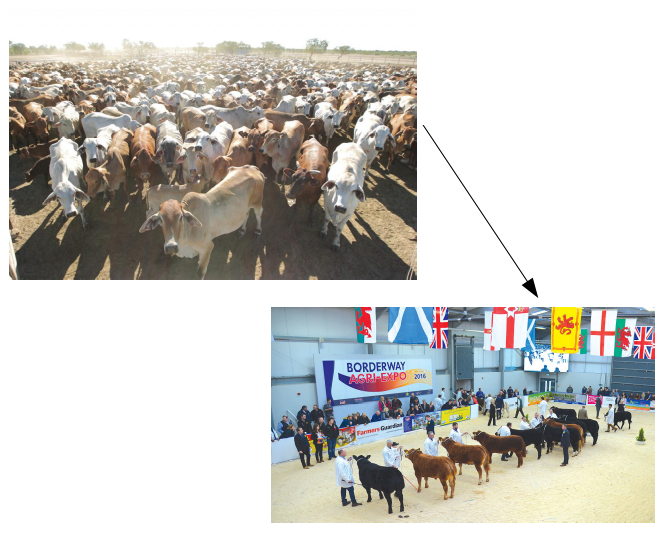
\includegraphics{odg/bestanimal.png}

\note{
\noindent\textbf{Notes}:
\begin{itemize}
\item 
\end{itemize}
}

\end{frame}

\begin{frame}{Phenotypes and Genotypes}
\protect\hypertarget{phenotypes-and-genotypes}{}

\[
P = G + E
\]

where \(P\) and \(E\) are observed and \(G\) is unknown

\note{
\noindent\textbf{Notes}:
\begin{itemize}
\item 
\end{itemize}
}

\end{frame}

\begin{frame}{Improving Animal Populations}
\protect\hypertarget{improving-animal-populations}{}

\begin{itemize}
\tightlist
\item
  Improvement via breeding \(\rightarrow\) long-term
\item
  Two tools
\end{itemize}

\begin{enumerate}
\tightlist
\item
  selection

  \begin{itemize}
  \tightlist
  \item
    process to determine parents of next generation
  \item
    natural selection in wildlife and livestock
  \item
    artificial selection in livestock: fix a goal and rank
  \end{itemize}
\item
  mating

  \begin{itemize}
  \tightlist
  \item
    which animal is bred to which
  \item
    extreme
  \item
    complementary
  \item
    heterosis - crossbreeding
  \end{itemize}
\end{enumerate}

\note{
\noindent\textbf{Notes}:
\begin{itemize}
\item 
\end{itemize}
}

\end{frame}

\begin{frame}{Statistics}
\protect\hypertarget{statistics}{}

\begin{itemize}
\tightlist
\item
  BLUP
\item
  Bayesian methods
\end{itemize}

\note{
\noindent\textbf{Notes}:
\begin{itemize}
\item 
\end{itemize}
}

\end{frame}

\begin{frame}{Computer Science}
\protect\hypertarget{computer-science}{}

\begin{itemize}
\tightlist
\item
  Methods have been developed in 1940's - 1950's
\item
  Progress occured later
\item
  Development of cheap computing power
\end{itemize}

\note{
\noindent\textbf{Notes}:
\begin{itemize}
\item 
\end{itemize}
}

\end{frame}

\begin{frame}{Milk Yield}
\protect\hypertarget{milk-yield}{}

\begin{figure}
\centering
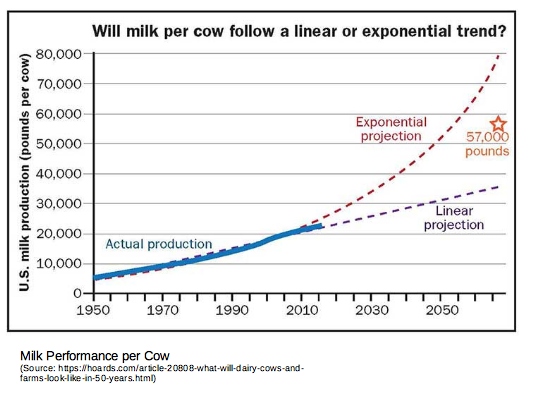
\includegraphics{odg/milkcompperf.png}
\caption{Yearly Milk Yield per Cow in the USA}
\end{figure}

\note{
\noindent\textbf{Notes}:
\begin{itemize}
\item 
\end{itemize}
}

\end{frame}

\begin{frame}{Computer Performance}
\protect\hypertarget{computer-performance}{}

\begin{figure}
\centering
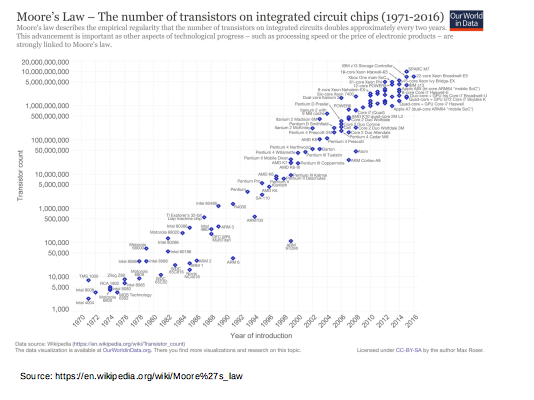
\includegraphics{odg/moorelaw.png}
\caption{Computing Performance According To Moore's Law}
\end{figure}

\note{
\noindent\textbf{Notes}:
\begin{itemize}
\item 
\end{itemize}
}

\end{frame}

\end{document}
